% ------------------------------------------------------------------------------
% TYPO3 Version 10.0 - What's New (English Version)
%
% @author	Michael Schams <schams.net>
% @license	Creative Commons BY-NC-SA 3.0
% @link		http://typo3.org/download/release-notes/whats-new/
% @language	English
% ------------------------------------------------------------------------------

\section{Wijzigingen voor Integrators}
\begin{frame}[fragile]
	\frametitle{Wijzigingen voor Integrators}

	\begin{center}\huge{Hoofdstuk 3:}\end{center}
	\begin{center}\huge{\color{typo3darkgrey}\textbf{Wijzigingen voor Integrators}}\end{center}

\end{frame}

% ------------------------------------------------------------------------------
% TYPO3 Version 10.0 - Breaking Changes

\begin{frame}[fragile]
	\frametitle{Wijzigingen voor Integrators}
	\framesubtitle{Brekende wijzigingen}

	\small
		Integrators, let op: In TYPO3 v9 is wat PHP-code, TSconfig, TypoScript
		opties en voorwaarden, alsook taakplannertaken aangemerkt als verouderd.

		\vspace{0.2cm}

		Volgens het \textbf{verouderingsbeleid} van TYPO3 worden deze componenten
		gewijzigd of verwijderd in TYPO3 v10.0.

		\vspace{0.2cm}

		Schakel de verouderingslog in, test alles zorgvuldig en bekijk de log om
		mogelijke problemen te vinden. Gebruik de ingebouwde
		\href{https://docs.typo3.org/m/typo3/reference-coreapi/master/en-us/ApiOverview/ExtensionScanner/Index.html}{Extensiescanner}
		om een compleet overzicht te krijgen van incompatibele zaken in extensies.

	\normalsize

\end{frame}

% ------------------------------------------------------------------------------
% Feature | 78432 | Add log message for Switch User action

\begin{frame}[fragile]
	\frametitle{Wijzigingen voor Integrators}
	\framesubtitle{Gebruikerswissel in Backend}

	\begin{itemize}
		\item In de log is terug te vinden als een admin gebruiker wisselt naar een andere backend-gebruiker:
	\end{itemize}

	\begin{figure}
		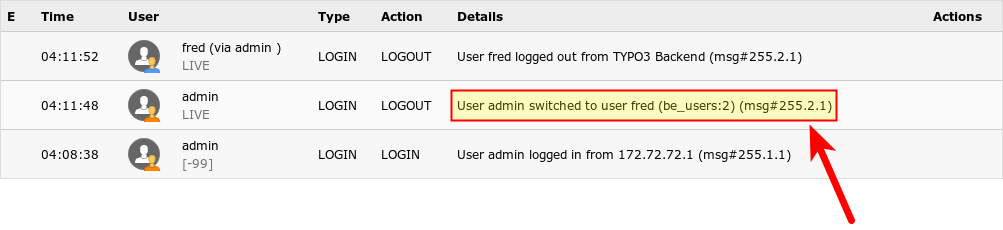
\includegraphics[width=0.90\linewidth]{ChangesForIntegrators/78432-SwitchUserActionLogMessage.png}
	\end{figure}

\end{frame}

% ------------------------------------------------------------------------------
% Feature | 83734 | Add support for current page in configcache
% Breaking | 88564 | PageTSconfig setting TSFE.constants removed
% Breaking | 88657 | Popup configuration in FormEngine dropped

\begin{frame}[fragile]
	\frametitle{Wijzigingen voor Integrators}
	\framesubtitle{Wijzigingen in TypoScript}

	\begin{itemize}
		\item TypoScript eigenschap \texttt{config.cache} ondersteunt het sleutelwoord
			"\texttt{current}" om te refereren aan de huidige pagina. Voorbeeld:\newline
			\smaller\texttt{config.cache.all = fe\_users:current}\normalsize

		\item De optie \texttt{TSFE.constants} in Page/User TSconfig is verwijderd.

			\begin{itemize}\smaller
				\item[\ding{228}] Gebruik TypoScript voorwaarden  in setup/constants en gebruik correcte configuratie in bestand \texttt{ext\_localconf.php}.
			\end{itemize}

		\item De volgende twee opties om de maat van een popup-venster in te stellen zijn verwijderd:

			\begin{itemize}
				\item \texttt{options.popupWindowSize}
				\item \texttt{options.rte.popupWindowSize}
			\end{itemize}

	\end{itemize}

\end{frame}

% ------------------------------------------------------------------------------
% Breaking | 88640 | Database field sys_template.nextLevel and TypoScript sublevel inheritance removed
% Task | 88755 | Remove POST option from typolink.addQueryString

\begin{frame}[fragile]
	\frametitle{Wijzigingen voor Integrators}
	\framesubtitle{Wijzigingen in TypoScript}

	\begin{itemize}
		\item Het database-veld \texttt{nextLevel} van de database-tabel
			\texttt{sys\_template} zijn verwijderd.

			\begin{itemize}\smaller
				\item[\ding{228}] Vervang het record (het UID is opgeslagen in het veld \texttt{nextLevel}) met een voorwaarden om TypoScript toe te voegen voor onderliggende pagina's. Bijvoorbeeld: \texttt{[tree.level > 1]}
			\end{itemize}\normalsize

		\item De volgende waarden zijn \textbf{niet meer toegestaan}:

			\begin{itemize}\smaller
				\item \texttt{typolink.addQueryString.method = POST}
				\item \texttt{typolink.addQueryString.method = GET,POST}
				\item \texttt{typolink.addQueryString.method = POST,GET}
			\end{itemize}\normalsize

			\begin{itemize}\smaller
				\item[\ding{228}] Wijzig de waarden in TypoScript, Fluid en PHP naar \texttt{GET}.
			\end{itemize}\normalsize

	\end{itemize}

\end{frame}

% ------------------------------------------------------------------------------
% Breaking | 87583 | Remove obsolete APC Cache Backend implementation
% Breaking | 87558 | Consolidate extbase caches

\begin{frame}[fragile]
	\frametitle{Wijzigingen voor Integrators}
	\framesubtitle{Caches}

	% decrease font size for code listing
	\lstset{basicstyle=\tiny\ttfamily}

	\begin{itemize}
		\item Het caching raamwerk ondersteunt de \texttt{ApcBackend} niet meer

			\begin{itemize}\smaller
				\item[\ding{228}] Gebruik \textbf{APCu} in plaats daarvan - let op de "u".
			\end{itemize}

\begin{lstlisting}
OUD:
$GLOBALS['TYPO3_CONF_VARS']['SYS']['caching']['cacheConfigurations']['rootline']['backend'] =
\TYPO3\CMS\Core\Cache\Backend\ApcBackend::class;

NIEUW:
$GLOBALS['TYPO3_CONF_VARS']['SYS']['caching']['cacheConfigurations']['rootline']['backend'] =
\TYPO3\CMS\Core\Cache\Backend\ApcuBackend::class;
\end{lstlisting}

		\item Extbase caches \texttt{extbase\_reflection} en \texttt{extbase\_datamapfactory\_datamap}
			zijn samengevoegd naar een cache met de naam "\texttt{extbase}".

	\end{itemize}

\end{frame}

% ------------------------------------------------------------------------------
% Breaking | 87009 | Use multiple translation files by default in EXT:form

\begin{frame}[fragile]
	\frametitle{Wijzigingen voor Integrators}
	\framesubtitle{Formulierraamwerk}

	% decrease font size for code listing
	\lstset{basicstyle=\tiny\ttfamily}

	\begin{itemize}
		\item De volgende optie is hernoemd:\newline
			\small\texttt{translationFile} \textrightarrow\hspace{0.1cm}\texttt{translationFiles}\normalsize
		\item De standaard taalbestanden zijn nu geregistreerd in index 10:

			\begin{itemize}
				\item \texttt{EXT:form/Resources/Private/Language/locallang.xlf}
				\item \texttt{EXT:form/Resources/Private/Language/Database.xlf}
			\end{itemize}

		\item Maatwerk YAML configuratiebestanden moeten bijgewerkt worden.

\begin{lstlisting}
OUD:
translationFile: path/to/locallang.xlf

NIEUW:
translationFiles:
  20: path/to/locallang.xlf
\end{lstlisting}

	\end{itemize}

\end{frame}

% ------------------------------------------------------------------------------
% xxxxx | Cache Storage Type

\begin{frame}[fragile]
	\frametitle{Wijzigingen voor Integrators}
	\framesubtitle{Cache opslagtype (1)}

	\begin{itemize}

		\item TYPO3 heeft een flexibel cachesysteem met een standaard configuratie
			die ideaal is in de meeste gevallen.
		\item Het opslagtype can nu geconfigureerd worden om de caches af te regelen en
			prestaties op specifieke omgevingen te verhogen.

			\begin{itemize}
				\item Kies de \textbf{database} storage voor standaardomgevingen
					of als bijvoorbeeld een netwerkbestandssysteem (NFS) gebruikt wordt,
				\item Kies het \textbf{bestandssysteem} als een gedistribueerde database wordt gebruikt.
				\item Kies \textbf{maatwerk cache-instellingen} om de opslag voor elke cache apart af te regelen.
			\end{itemize}

		\item Voor complexere installaties kunnen geheugen caches zoals
			\href{https://redis.io/}{Redis}
			of
			\href{https://memcached.org/}{Memcached}
			overwogen worden.

	\end{itemize}

\end{frame}

% ------------------------------------------------------------------------------
% xxxxx | Cache Storage Type

\begin{frame}[fragile]
	\frametitle{Wijzigingen voor Integrators}
	\framesubtitle{Cache opslagtype (2)}

	\begin{itemize}

		\item Backend: \textbf{MAINTENANCE} \ding{223}\hspace{0.1cm}\textbf{Settings} \ding{223}\hspace{0.1cm}\textbf{Cache}:
		\end{itemize}

	\begin{figure}
		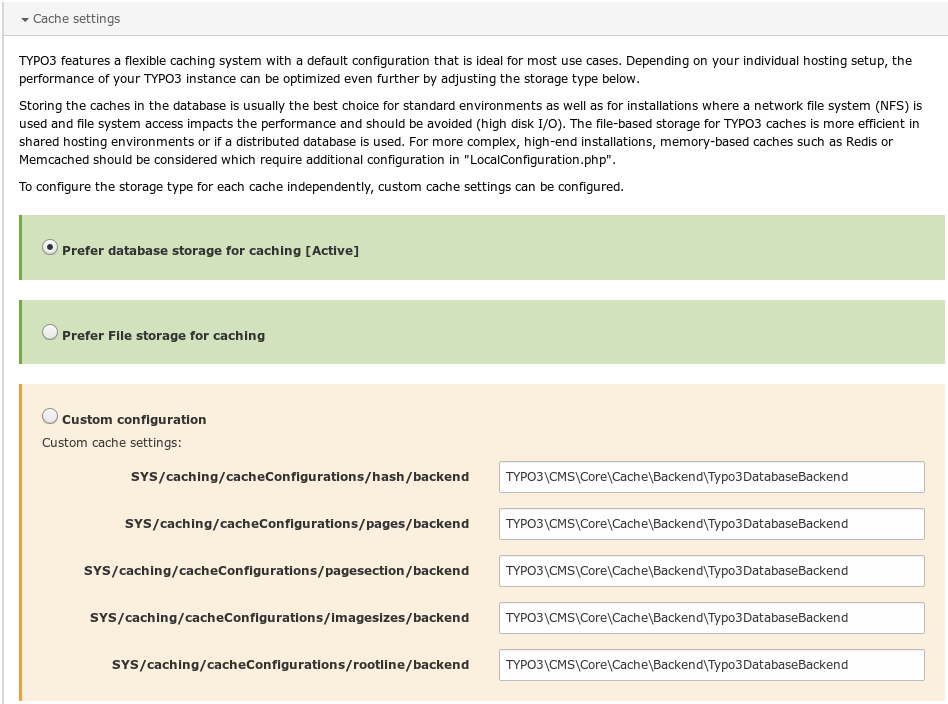
\includegraphics[width=0.60\linewidth]{ChangesForIntegrators/xxxxx-CacheStorageType.png}
	\end{figure}

\end{frame}

% ------------------------------------------------------------------------------
% 87499 | Drop extensions "taskcenter" and "sys_action" from core

\begin{frame}[fragile]
	\frametitle{Wijzigingen voor Integrators}
	\framesubtitle{Taakcentrum en \texttt{EXT:sys\_action}}

	\begin{itemize}

		\item De systeemextensies \texttt{EXT:taskcenter} en \texttt{EXT:sys\_action}
			zijn uit de core verwijderd.

		\item Ze zijn nu beschikbaar als aparte extensies in
			\href{https://extensions.typo3.org/}{TER}
			en op
			\href{https://github.com/FriendsOfTYPO3}{GitHub}.

		\item Let op het
			\href{https://typo3.org/community/teams/typo3-development/initiatives/typo3-dashboard-initiative/}{Dashboard Initiatief}
			voor een nieuw en veel beter alternatief.

	\end{itemize}

\end{frame}

% ------------------------------------------------------------------------------
% Feature | 88648 | Define Twitter Card Type In Page Properties
% Important | 86577 | Query parameters are now included in canonicalized URLs

\begin{frame}[fragile]
	\frametitle{Wijzigingen voor Integrators}
	\framesubtitle{Diversen}

	% decrease font size for code listing
	\lstset{basicstyle=\tiny\ttfamily}

	\begin{itemize}

		\item Het type Twitter Card kan nu gekozen/geconfigureerd worden.
			Deze optie zorgt voor de metatag \texttt{twitter:card} in de frontend.

\begin{lstlisting}
page {
  meta {
    twitter:card = summary_large_image
    twitter:card.replace = 1
  }
}
\end{lstlisting}

		\item Alleen parameters die nodig zijn om de cHash te berekenen worden standaard meegenomen in genormaliseerde URL's.
			Extra parameters kunnen nu geconfigureerd worden:

\begin{lstlisting}
$GLOBALS['TYPO3_CONF_VARS']['FE']['additionalCanonicalizedUrlParameters'].
\end{lstlisting}

		\smaller
			Let op: voeg alleen parameters toe die de inhoud van de pagina wijzigen. Anders zien zoekmachines het wellicht als dubbele inhoud.
		\normalsize

	\end{itemize}

\end{frame}

% ------------------------------------------------------------------------------
% Breaking | 88681 | Import Of PHP Files In Import Export Files Removed
% Breaking | 88500 | RTE image handling functionality dropped
% Breaking | 81950 | Remove leftover workspaces unpublishing functionality

\begin{frame}[fragile]
	\frametitle{Wijzigingen voor Integrators}
	\framesubtitle{Diversen}

	% decrease font size for code listing
	\lstset{basicstyle=\tiny\ttfamily}

	\begin{itemize}

		\item Bij het importeren van XML-data met \texttt{EXT:impexp} wordt het Patroon voor het weigeren van bestanden gebruikt en
			weigert nu bijvoorbeeld PHP bestanden.

		\item Ondersteuning voor afbeeldingen in de RTE is compleet verwijderd.
			Voor ondersteuning van afbeeldingen in CKEditor kan bijv. \texttt{EXT:rte\_ckeditor\_image} gebruikt worden.

		\item Een eigenschap binnen werkruimtes voor het \textit{de-publiceren} van records is verwijderd in v10
			(inclusief databaseveld \texttt{sys\_workspace.unpublish\_time}). Deze functie was uitgeschakeld
			in TYPO3 v4.5 en niet meer gebruikt of beschikbaar gesteld door TYPO3.

	\end{itemize}

\end{frame}

% ------------------------------------------------------------------------------
% Breaking | 88772 | JavaScript script tags omit type=text/javascript in HTML5
% Remove system extension EXT:rsaauth
% Remove system extension EXT:fe_edit

\begin{frame}[fragile]
	\frametitle{Wijzigingen voor Integrators}
	\framesubtitle{Diversen}

	% decrease font size for code listing
	\lstset{basicstyle=\tiny\ttfamily}

	\begin{itemize}

		\item Bij het maken van HTML5 output krijgen \texttt{<script>} tags geen
			\texttt{type="text/javascript"} attribuut meer.

		\item Dit kan in TypoScript weer ingeschakeld worden indien nodig:

\begin{lstlisting}
page {
  includeJS {
    myfile = EXT:example/Resources/Public/JavaScript/myfile.js
    myfile.type = text/javascript
  }
}
\end{lstlisting}

		\item De volgende verouderde systeemextensies zijn verwijderd:

			\begin{itemize}
				\item \texttt{EXT:rsaauth}
				\item \texttt{EXT:fe\_edit}
			\end{itemize}

	\end{itemize}

\end{frame}

% ------------------------------------------------------------------------------
